\chapter{An Approach to Intention-oriented Organizational Modeling}
\label{chap:approach}
This chapter describes in detail about the technical approach that has been taken to solve the problem mentioned in the Section \ref{sec:problemstatement} of Chapter \ref{chap:introduction} and to satisfy all of the requirements mentioned in the Section \ref{sec:requirementssupoorting} of Chapter \ref{chap:analysis}. The first section of this chapter provides an overview of the intention-oriented organizational modeling process. The second section discusses in detail second phase (P2) of the InProXec method, i.e., Model Informal Processes. The third section discusses in detail about the \textit{top-down approach}, which helps to realize the intention-oriented organizational modeling. The fourth section discusses the design methodology followed to realize this approach as a web-based modeling tool. 

%%%%%%%%%%%%%%%%%%%%%%%%%%%%%%%%%%%%%%%%%%%%%%%%%%%%%%%%%%%%%%%%%%%%%%%%%
\section{Overview of the Modeling Process}
\label{sec:overviewmodelingprocess}
%%%%%%%%%%%%%%%%%%%%%%%%%%%%%%%%%%%%%%%%%%%%%%%%%%%%%%%%%%%%%%%%%%%%%%%%%
The main focus of this approach is to develop a web-based modeling tool that satisfy all of the requirement of intention-oriented organizational modeling and can be used by business experts to model informal processes, intentions, strategies and capabilities. Also in this thesis work, the scope of modeling is limited only to the descriptive type of modeling i.e., models that describe processes declaratively by providing only information about what has to be done. As we mentioned before, the resource definitions required for the modeling tool is made available from the first phase P1 of the InProXec approach. Business experts develop descriptive models through the developed modeling tool using these resource models to achieve main intention that contains strategies. The reason for following descriptive modeling approach is due to the fact that models reuse descriptive data and these stored models provides means of execution for the phase P3 of InProXec. The models developed through this approach provides necessary concepts and elements for intention-oriented organizational modeling. Resources are abstract description which are made concrete during initialization of an instance. There are also participant specific views based on the participating resources' role. For example, based on the privilege provided to a participant he can view, edit, own or follow the instances. Initializing resource-centric models requires \textit{acquiring} and engaging interrelated resources \cite{Sungur2015} which is explained in a detailed way in the following sections of this chapter. 

%%%%%%%%%%%%%%%%%%%%%%%%%%%%%%%%%%%%%%%%%%%%%%%%%%%%%%%%%%%%%%%%%%%%%%%%%
\section{Second Phase of InProcXec - Model Informal Process}
\label{sec:informalprocessmodeling}
%%%%%%%%%%%%%%%%%%%%%%%%%%%%%%%%%%%%%%%%%%%%%%%%%%%%%%%%%%%%%%%%%%%%%%%%%
This approach of Informal Process Modeling is directed towards modeling the informal process based on their intentions rather than their activities.  Since this phase is a part of InProXec method, the properties and requirements of informal process described in previous approaches \cite{Sungur2014a,Sungur2015} also applies to informal process modeling phase. The developed system serves as an holistic web based modeling tool to create, view and update all the associated elements of informal process like contexts, intentions, capabilities, strategies and resources. Also, from our detailed explanation in previous sections about the importance of resources in organizational modeling and along with the fact that phase P2 receives resource definitions as input from phase P1 of InProXec method, we can apprehend that resource definitions are the lowest level in the hierarchy of intention-oriented organizational modeling approach. The sequence of steps to be carried out using the developed modeling tool has been shown in the Figure \ref{fig:processdiagram}. 

\begin{figure}
	\centering
	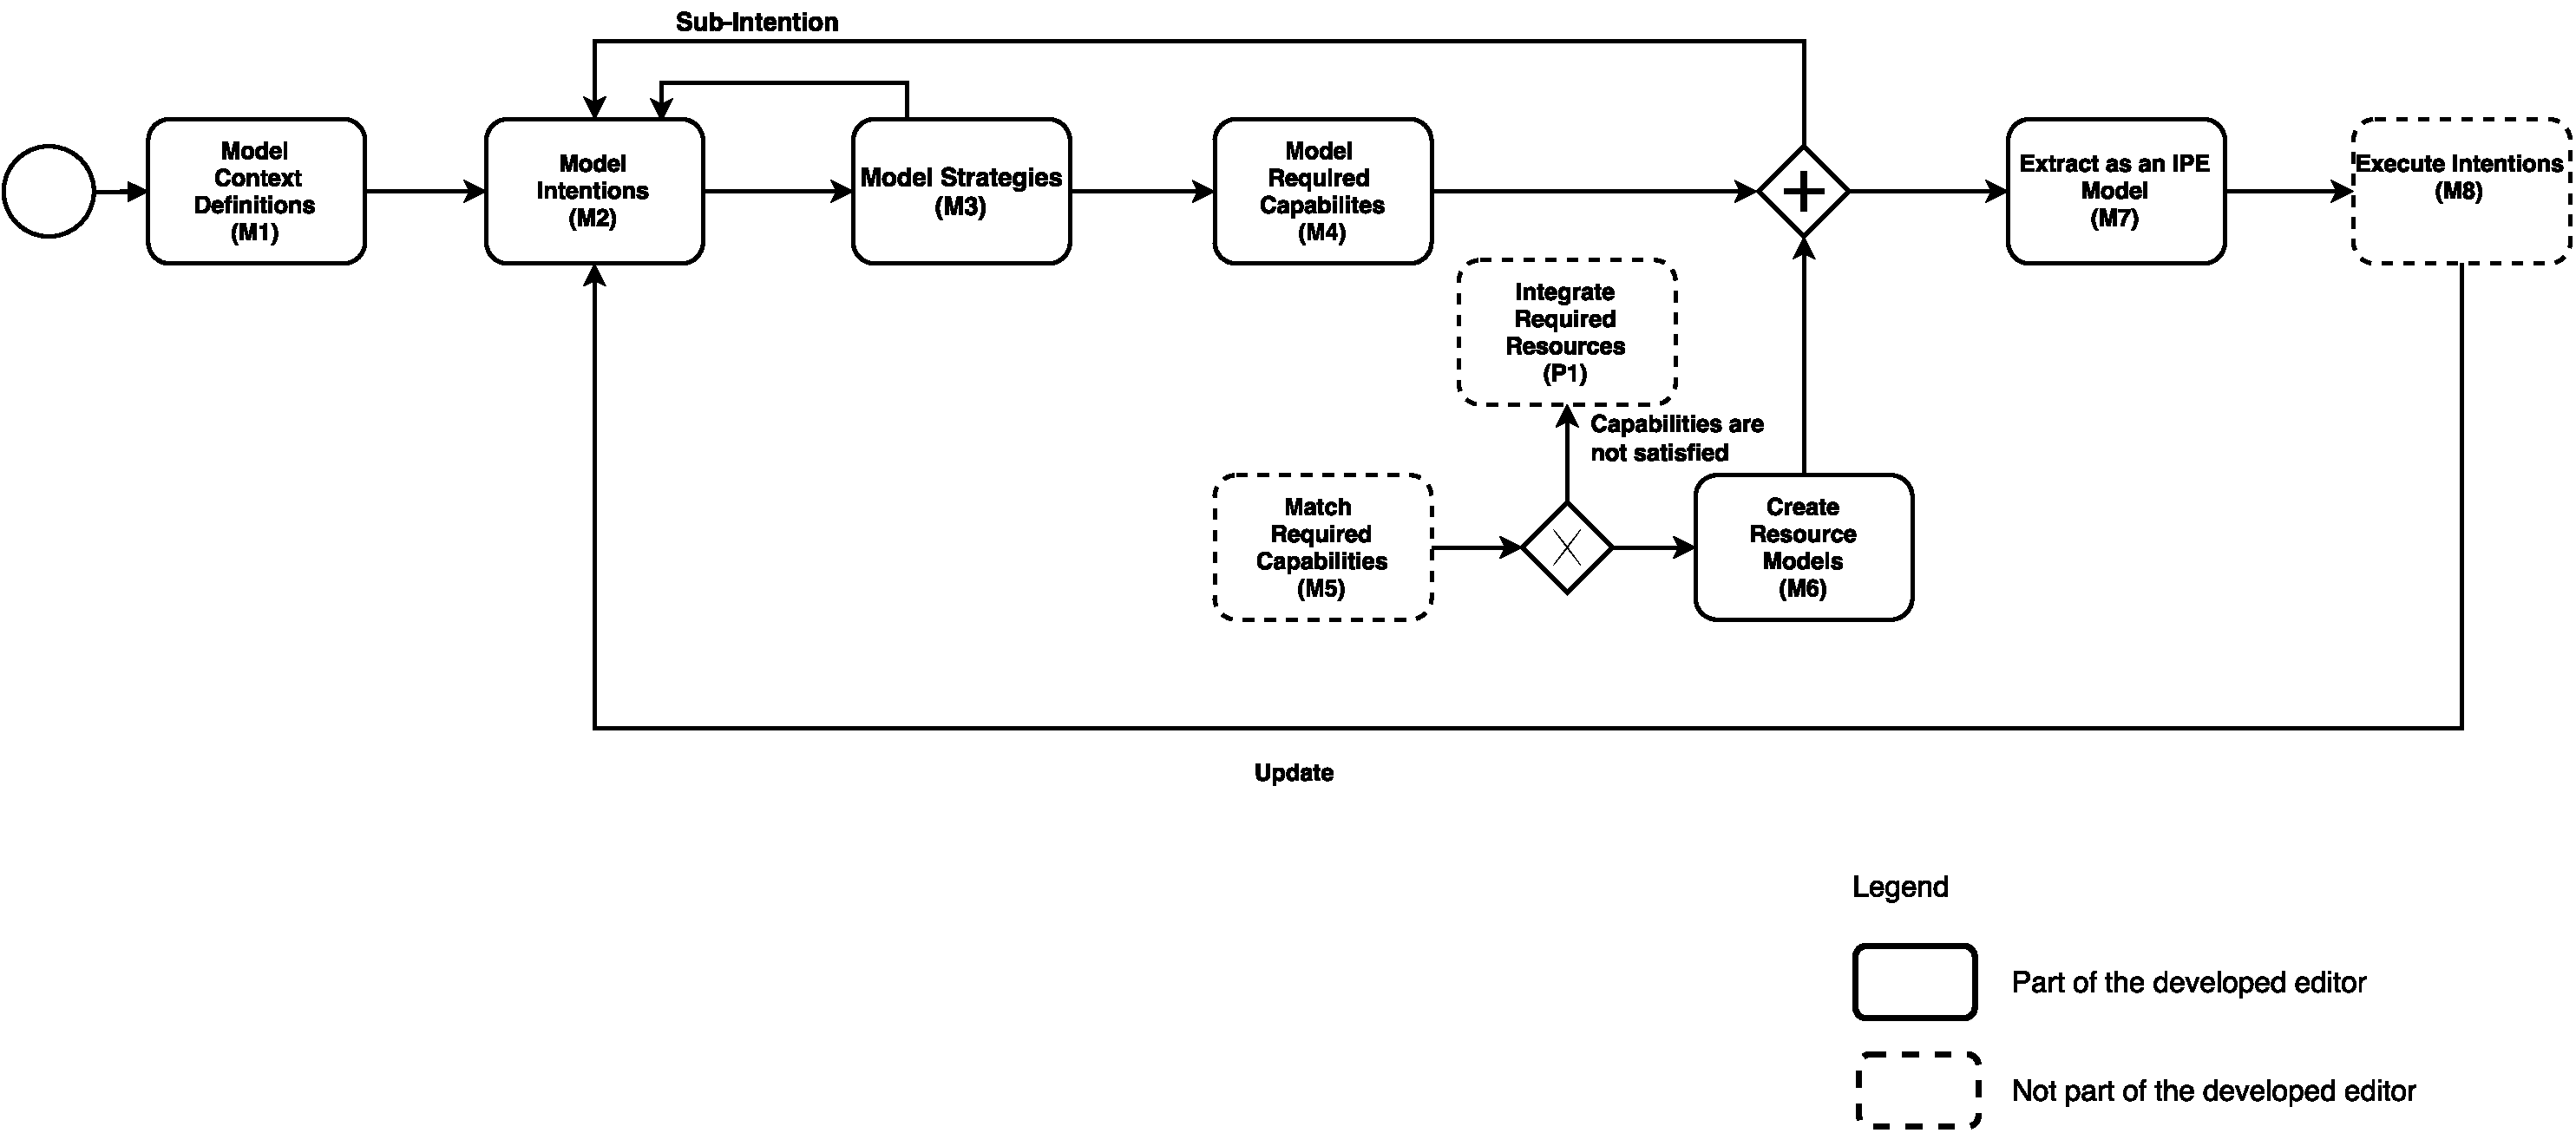
\includegraphics[width = \textwidth]{processmodeling.pdf}
	\caption{Steps of Model Informal Process}
	\label{fig:processdiagram}
\end{figure}

\subsubsection{Model Context Definitions (M1)}  
The first step is to model context definitions, where we can model both (1) basic properties like name and namespace of a context definition and (2) entity specific properties like contained contexts, entity definitions, etc., of a context definition.  

\subsubsection{Model Intentions (M2)}  
Similar to context definition modeling (M1), the second step (M2) is to model intentions. The context definitions created in step M1 can be used to specify initial and final contexts of an intention. Intentions can contain related intentions such as (1) sub-intentions and (2) contradicting intentions. These type of sub intentions and contradicting intentions are also modeled as intentions in this step and their type of relation to a specific intention are mentioned. Intentions are defined hierarchically, which can contain and extend intentions. It is depicted by a double circle in organizational modeling notations. The sub-intentions are refined starting from main intention. Intentions are associated with strategies. Strategies, required to achieve an intention are added to entity specific properties of intention as achieving strategies in this step.

\subsubsection{Model Strategies (M3)}  
Once intentions are identified and modeled, the third step (M3) is modeling of strategies to achieve a specific intention. As mentioned earlier in the Section \ref{sec:entitytypesrepresentation}, an intention can have multiple strategies.  A strategy is a method or plan chosen to bring desired results, such as achievement of an intention or solution to a problem. Strategies are associated with capabilities. The capabilities required by strategy are added to entity specific properties of strategy in this step. 

\subsubsection{Model Required Capabilities (M4)}  
After modeling of strategies, capabilities required to achieve an intention in a specific strategy is modeled. A strategy can require multiple capabilities. A capability is an ability to provide business values like software applications, resources and potential of the actor to make decisions even in changing situations \cite{Stirna2012}. Capability describes the ability provided by a resource or required by an intention. The performers of an informal process should posses certain skills and roles to achieve the intention. These type of required skills are modeled during this step.

\subsubsection{Create Resource Models (M6)}  
After matching the resources and capabilities i.e after finding the correct resource that has the capability to carry out the process, the resource models are created. The need for modeling a new intention may arise in parallel during modeling of resources. This has been explained with a suitable example in the following Chapter \ref{chap:motivatingScenario}.  A resource can be a people or tool those/that drive towards the successful execution of the process. It is key for achieving specified process intentions. In the context of this work, the definition of organizational resources refers not only the entities that are capable of doing work but also entities that have an impact on the outcome of the processes, e.g., software tools, human performers, data etc.      

\subsubsection{Extract as an IPE Model (M7)}  
After the completion of above mentioned steps, the modeled entities can be extracted as an IPE model which can be reused. 

The steps matching of required organizational capabilities (M5) that are satisfied by resource models and integration of required resources (P1) are not part of the current functioning tool. If there is no suitable matching capability, then phase P1 of InProXec can be carried out again until a matching capability is found. If capabilities are satisfied resource models can be created. The created resource models (M6) along with modeled capabilities can be extracted as an IPE Model (M7) which can be provided as input for the next step achieve intentions (M8). After achieving an intention, the status of intention is updated inside the specific intentions's property. 

%%%%%%%%%%%%%%%%%%%%%%%%%%%%%%%%%%%%%%%%%%%%%%%%%%%%%%%%%%%%%%%%%%%%%%%%%
\section{A Top-down Modeling Approach}
\label{sec:topdownapproach}
%%%%%%%%%%%%%%%%%%%%%%%%%%%%%%%%%%%%%%%%%%%%%%%%%%%%%%%%%%%%%%%%%%%%%%%%%
As we mentioned earlier, the modeling approach in our context is descriptive modeling approach which starts from top level intention and refines modeling until the operational bottom level is reached. Hence, it is called top-down modeling approach. The purpose of selecting top-down modeling approach is because based on the suggestions provided in the literatures \cite{Mandic2010, Bider2005,Sungur2016}, that value of intention in the top of hierarchy propagates till the lower levels and helps in making investment-related decisions while at the same time integrating cost and benefit estimates from all levels. Moreover, by creating declarative models using top-down modeling approach. Models are easily changeable as they are decoupled from their operational terms. Such declarative approaches provide more flexibility and enable easier to change the business process models. The integration of declarative models using top-down modeling approach, also provides coupling of cost-benefit and strategy achievability estimation with operationally measurable business intention and supports the evaluation of business intention's success and the effectiveness of the chosen strategies. In the Figure \ref{fig:topdownapproach}, it is shown how this modeling approach starts modeling from top level intentions and does modeling until the operational lower level is reached and how the organizational modeling elements are associated with each other. 

\begin{figure}
	\centering
	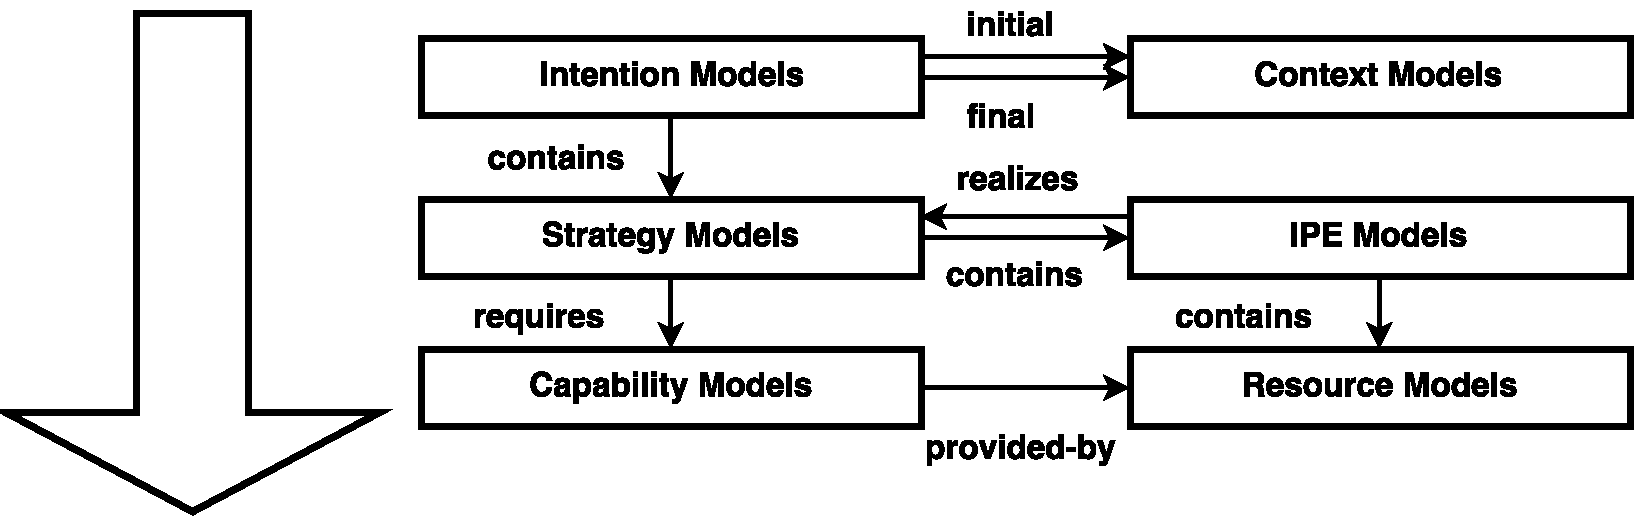
\includegraphics[width=\textwidth]{TopDownApproach.pdf}
	\caption{Intention-oriented Organizational Modeling - A Top down Modeling Approach}
	\label{fig:topdownapproach}
\end{figure}

The approach is evaluated based on the derived requirements in the Section \ref{sec:requirementssupoorting} of Chapter \ref{chap:analysis} as follows :

\textit{Organizational Intention Transparency} (R1) : From the Figure \ref{fig:topdownapproach}, one could understand that (1) intentions are refinable and as per the current design of the approach, (2) organizational members can view the intentions at different levels. Thus, requirement R1 is satisfied by the approach as it satisfies all of the pre-requisites. 

\textit{Organizational Strategy-based Cost Estimation} (R2) : During the modeling phase itself, business executives can make decisions based on the strategy cost estimation. In this approach, (1) resources are associated with cost and (2) the cost estimation of strategies include all its low level structures. Thus, requirement R2 is satisfied by the approach as it satisfies all of the pre-requisites. 

\textit{Organizational Strategy Achieve-ability Estimation} (R3) : Similar to requirement R2, strategy achievability estimation based on strategy's association with valid capability is also estimated during modeling phase itself. In this approach (1) a capability is considered as valid only when it is associated with matching resource and (2) from the Figure \ref{fig:topdownapproach}, one could understand how independent informal process realizes strategy. Thus, requirement R3 is satisfied by the approach as it satisfies all of the pre-requisites.

\textit{Intention Oriented Working Style} (R4) : This approach (1) satisfies requirement R1 and (2) when modeling through this approach members require understanding of intention and its associated elements for successfully achieving the main intention. Thus, requirement R4 is satisfied by the approach as it satisfies all of the pre-requisites.

\textit{Participative Organizational Modeling} (R5) : This approach (1) satisfies requirement R1 and  (2) intentions are modeled collaboratively based on input received from different members of the organization. Thus, requirement R4 is satisfied by the approach as it satisfies all of the pre-requisites. 



